\section{Experimental Studies}
\label{sec-expt}

In this section, we conducted two sets of experiments to evaluate (1) the performance of our visual processing module, (2) the accuracy of our inference module, and (3) the overall performance of our approach. 

\stitle{Experimental Setting}. %We report settings of experimental studies. 

\etitle{DataSet}. We used two datasets: (1) \kw{Soccer} dataset that we annotated; and (2) X dataset from~\cite{}. We extracted images with subjects of golf and tennis (report Statistics about the dataset). We split \kw{Soccer} (resp. X) data into two parts:{\em  I} (one third) and {\em II} (two thirds), and used {\em II} as training data, and {\em I} as testing data. 

\etitle{Queries}. We used two sets of questions: (1) the set of questions given in Table~\ref{table:questions} for \kw{Soccer} dataset; and (2) another set of questions listed in Table~\ref{} for X dataset. 

\begin{table}[thb] 
\footnotesize
\begin{tabular}{|l|l|l|}
\hline
Id & Question                                           & Difficulty \\ \hline
%$Q_{nl_1}$  & Who is this image about?                         & Hard       \\ \hline
$Q_{nl_1}$  & Who is holding the soccer?                         & Easy       \\ \hline
$Q_{nl_2}$  & What is the uniform color of the referee?           & Easy       \\ \hline
$Q_{nl_3}$  & Is there any referee in the image?                 & Easy       \\ \hline
$Q_{nl_4}$  & Which team does the goalkeeper belong to?          & Medium       \\ \hline
$Q_{nl_5}$  & Who is the defending team?                         & Medium       \\ \hline
$Q_{nl_6}$  & Which part of the field are the players being now? & Hard       \\ \hline
$Q_{nl_7}$  & How many players are there in the image?           & Hard     \\ \hline
$Q_{nl_8}$  &            &      \\ \hline
$Q_{nl_9}$  &            &      \\ \hline
$Q_{nl_10}$  &            &      \\ \hline
\end{tabular} 
\caption{A set of questions} \label{table:questions}
\end{table}




\subsection{Performance of Visual Processing}

{\color{red} Peixi, please report your results with details here.}



\begin{figure}[tb!]
\centering
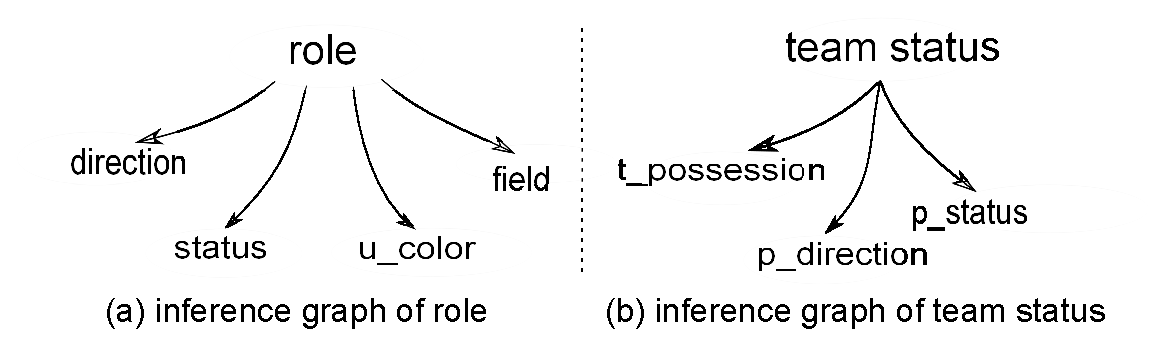
\includegraphics[width=\columnwidth]{./figure/PredictNB.eps}
\vspace{-2ex}
\caption{Inference Graphs}
\vspace{-2ex}
\label{fig:inferG}
\end{figure}

\subsection{Effectiveness of Inference} 

\stitle{Accuracy of Role}. Only report results with Reinforcement learning 

\stitle{Accuracy of Team-Status}. Only report results with Reinforcement learning 

\stitle{Accuracy of Kick-Off}. {\color{red} SHOW INFERENCE GRAPH AND RESULT TABLE!}

\stitle{Accuracy of Penalty Kick}. {\color{red} SHOW INFERENCE GRAPH AND RESULT TABLE!}

\stitle{Accuracy of Corner Kick}. {\color{red} SHOW INFERENCE GRAPH AND RESULT TABLE!}

\stitle{Accuracy of Attacking Free Kick}. {\color{red} SHOW INFERENCE GRAPH AND RESULT TABLE!}

\stitle{Accuracy of Balls}. {\color{red} Over new dataset. SHOW INFERENCE GRAPH AND RESULT TABLE!}

\subsection{Overall Performance}
\label{sec-overall-performance}

We compared the following state-of-the-art methods: X1, X2 and X3 with ours. 